\documentclass[letter,12pt]{article}
\usepackage[utf8]{inputenc}
\usepackage{times}
\usepackage[letterpaper, margin=1in]{geometry}
\usepackage{graphicx}
\usepackage{amsmath,amssymb}
\usepackage{textgreek}
\usepackage{natbib}
\usepackage{float}
\bibliographystyle{aasjournal}

\title{\vspace*{-2cm}Direct detection of the bulk neutral IGM at reionization}
\author{PI: B.~Mobasher 2019A\_U223}
\date{}
\newcommand{\lya}{Ly\textalpha}
\newcommand{\HI}{H\,{\sc i}}
\newcommand{\cii}{C\,{\sc ii}}
\newcommand{\oii}{O\,{\sc ii}}
\newcommand{\oiii}{O\,{\sc iii}}
\newcommand{\stromgren}{Str\"{o}mgren}
\newcommand{\apj}{ApJ}
\newcommand{\aj}{AJ}
\newcommand{\aap}{A\&A}
\newcommand{\nat}{Nature}
\newcommand{\mnras}{MNRAS}

\begin{document}

\maketitle

\section{Scientific Justification}

Observations of the CMB put the epoch of reionization of the intergalactic
medium (IGM) at \(z=6.4\textup{--}9.7\) \citep{2016A&A...596A.108P}. There is
compelling evidence for some IGM neutrality at these redshifts in the spectra of
\textgamma-ray bursts (GRBs) and quasars \citep[e.g.][]{2006AJ....132..117F},
which show the anticipated flux suppression of the Gunn-Peterson trough. But an
unequivocal direct detection of the bulk neutral IGM gas itself still eludes us.

\textbf{We propose to make this key observation of reionization by detecting the
red damping wing of the IGM's hydrogen \lya\ absorption across the foreground of
a galaxy at \(z>7\).}

Because the IGM was not uniformly reionised, we cannot use just any object at
\(z>7\). We need a source that lies in a neutral IGM region at that
redshift. To exclude the possibility of a small intervening cloud,
we use a source extended over a large area, i.e.\ a resolved galaxy rather than
a quasar. A galaxy that is both bright enough and in an IGM-neutral
region at \(z>7\) is rare, since UV-bright sources will not only ionize an
extended volume around them, but also lie in massive halos near other
luminous sources. The characteristic signature of a galaxy with neutral IGM
absorption is a large (\(\sim\)10000\,km\,s\(^{-1}\)) red offset of the galaxy's
\lya\ break compared to its systemic redshift. Recently, we have found that the
reionization-epoch galaxy, A1689-zD1, has this signature and a deep MOSFIRE
observation would be able to detect the damping wing.

A1689-zD1 is a small (sub-L*), dusty galaxy. However, it is
gravitationally-lensed by a factor of 9 \citep{2008ApJ...678..647B}, making it
bright enough to be spectroscopically accessible. The systemic redshift is
\(z=7.132\) determined from detections of the \cii\ 158\,{\textmu}m and CO(3--2)
lines. However, the redshift determined from NIR spectroscopy with VLT/X-shooter
of the \lya\ spectral break is offset to the red by 14\,000\,km\,s\(^{-1}\),
i.e.\ X-shooter spectroscopy shows a break at about 1270\,\AA\ in the galaxy's
restframe instead of 1216\,\AA, indicating an extremely high column density
\lya\ absorption line with a strong red damping wing. Measuring such a \lya\
trough would be a clear detection of the bulk neutral IGM because the source is
extended and the absorber must have a very high column density
(\(\log{N_\mathrm{H\,\textsc{i}}}\sim23\)). Our proposal seeks to measure the
shape of this damping wing, and we need MOSFIRE on Keck to do it because it's
the most sensitive spectrograph in the world at 1\,{\textmu}m. X-shooter's
sensitivity is a factor of 4 lower in this region of the spectrum.


\subsection{A1689-zD1 and the redshift discrepancy}

A1689-zD1 was discovered as a HST \(z\)-band dropout \citep{} showing it to be a
\(z\) = 7--8 galaxy, gravitationally lensed by the galaxy cluster Abell\,1689.
We analysed the results of Cycle~0, 1, and 2 ALMA and VLT/X-shooter observations
\citep{watson15,2017MNRAS.466..138K} and found the galaxy to be dusty and
evolved and we retrieved a coarse optical/NIR spectrum (Fig.~1) that confirmed
spectroscopically the high redshift nature of the galaxy and located the break
redshift at \(z=7.5\pm0.2\). The break can only be due to \lya\ because of its
depth and the relatively blue slope of the continuum. While the break is clearly
visible in Fig.~1, the redshift uncertainty reflects that we needed to bin the
spectrum substantially to recover the continuum emission and the break lies
close to the region of least sensitivity for X-shooter---on the dichroic
between the VIS and NIR arms. Our ALMA observations in bands~6 and 7 showed a
clear detection of the source in dust continuum emission, with the HST and ALMA
images of the galaxy co-spatial---there is no significant offset
\citep{watson15,2017MNRAS.466..138K}.

In the ALMA Cycle~3 data we find a strong emission line with significant
velocity structure (Fig.~2). We infer this to be the \cii\,157.7\,{\textmu}m
emission line at a redshift \(z=7.132\). The line is bright, with a flux of
approximately 4\,Jy\,km\,s\(^{-1}\). The [C\,\textsc{ii}] identification gives a
flux consistent with expectations for this galaxy \citep{2011MNRAS.416.2712D}.
In our deep observations with GBT this year, we have detected a line at the
expected frequency and luminosity \citep{2010ApJ...724..957S} for CO(3--2),
confirming the systemic redshift, \(z=7.132\).

This redshift implies a \lya\ break at 989\,nm, strongly inconsistent
with our observed \lya\ break wavelength from VLT/X-shooter (Fig.~1), and lying
about 14\,000\,km/s from the best fit. While the spectral break redshift has a
conservative uncertainty of 0.2, the uncertainty space is highly non-linear and
a redshift of \(7.132\) is excluded. This is because the dichroic
region of the X-shooter spectrograph has particularly low signal-to-noise ratio,
but 989\,nm, where we expect \lya\ at \(z=7.312\), is in the good part of the
VIS arm and galaxy emission can be excluded there (Fig~1).


\subsection{A unique opportunity to detect the bulk IGM}

While modest velocity offsets with \lya\ \emph{in emission} are common due to
the resonant scattering of the emission line, very large discrepancies with the
absorption break are not expected and can only readily be explained except by a
very large, damped absorption line. A line with \(\log(N_{{\rm H\,I}}/{\rm
cm}^2)\simeq23\) at \(z=7.132\) would yield an apparent break in very low SNR
data at \(z\sim7.5\). We believe this is the damping wing of the neutral IGM
\citep[the Gunn-Peterson damping wing;][]{1998ApJ...501...15M}. Such a column
density is consistent with simulations of neutral gas densities in a reasonable
fraction of lines of sight at this redshift (Kaurov \& Gnedin 2015, ApJ 810,
154). The column cannot be associated with gas from the galaxy itself since the
galaxy would be completely dust obscured (\(A_V \sim 60\)), given the
dust-to-gas ratio for this galaxy \citep{watson15}, furthermore the column
density is about two orders of magnitude larger than damped \lya\ absorbers
(DLAs) observed in galaxy spectra to date. To have such a large column DLA in
this galaxy would require the DLA cloud to be pristine and to be foreground to
essentially the entire galaxy and would require a H\,\textsc{i} cloud of at
least the same mass as the galaxy gas mass. Such a cloud would be unstable to
self-gravity and would collapse in only a few million years. The only credible
explanation for the redshifting of the break is absorption by a large neutral
IGM component.

Evidence of a damping wing has been seen in two \(z>7\) quasars
\citep{2011Natur.474..616M,2018Natur.553..473B}, but suffer from a number of
caveats, most important of which is the possibility of a small local cloud
intercepting the line-of-sight, a caveat noted by both
\citeauthor{2011Natur.474..616M} and \citeauthor{2018Natur.553..473B} This
caveat also applies to GRBs \citep[e.g.][]{2009Natur.461.1254T}, but is a
possibility excluded in A1689-zD1 by the extended nature of the source.

A1689-zD1 represents a unique opportunity to detect the damping wing of the
neutral IGM during reionization. We therefore request a MOSFIRE observation of
the galaxy. The observation is designed to be deep enough to get a direct
detection of the IGM damping wing.  We have calculated the expected spectrum
using the MOSFIRE ETC (Fig.~1) and we can clearly discriminate a damping wing
compared to a sharp break and measure the column density in 16 hours exposure.

\clearpage

\begin{figure}[H]
  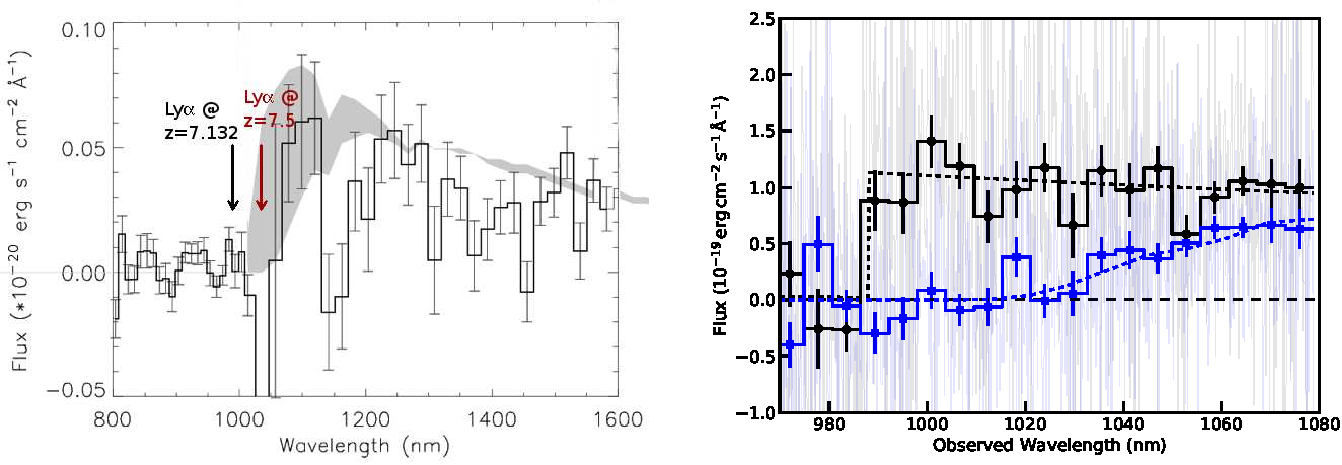
\includegraphics[width=1.0\textwidth,clip=]{NIR_new.pdf}
  \caption{\emph{Left}: VLT/X-shooter spectrum of Abell\,1689-zD1.  A break at
  \(z\sim7.5\) is apparent.
  The location of a simple \lya\ break if it were at the redshift of the
  [\cii]\,158\,\(\mu\)m line, \(z=7.132\), is indicated and is excluded
  by these X-shooter data.  The shaded area indicates the allowed 1\textsigma
  limits for the spectrum due to absorption by a DLA system fixed at \(z=7.132\)
  that would be required to explain the UV/FIR redshift discrepancy.  The NIR
  spectrum is strongly affected by atmospheric absorption bands.
  \emph{Right}: Simulation of the spatially integrated MOSFIRE spectrum based on
  galaxies absorbed by a
  \(\log(N_{{\rm H\,I}}/{\rm cm}^2)=23.1\) cloud (blue) and a standard IGM cut-off
  model (Meiksin 2006, MNRAS 365, 807, black).  The simulation uses the
  MOSFIRE ETC and accounts for sky emission and absorption lines as well as
  instrumental noise.  The lighter, thin lines are the unbinned spectra.  The
  heavy histograms are these same spectra binned.  We can clearly distinguish
  with these data between a sharp break and a large \lya\
  absorber both at the systemic redshift, \(z=7.132\) (models shown as dotted black and blue lines
  respectively) and we will be able to measure the effective column density.}
\end{figure}

\begin{figure}[H]
  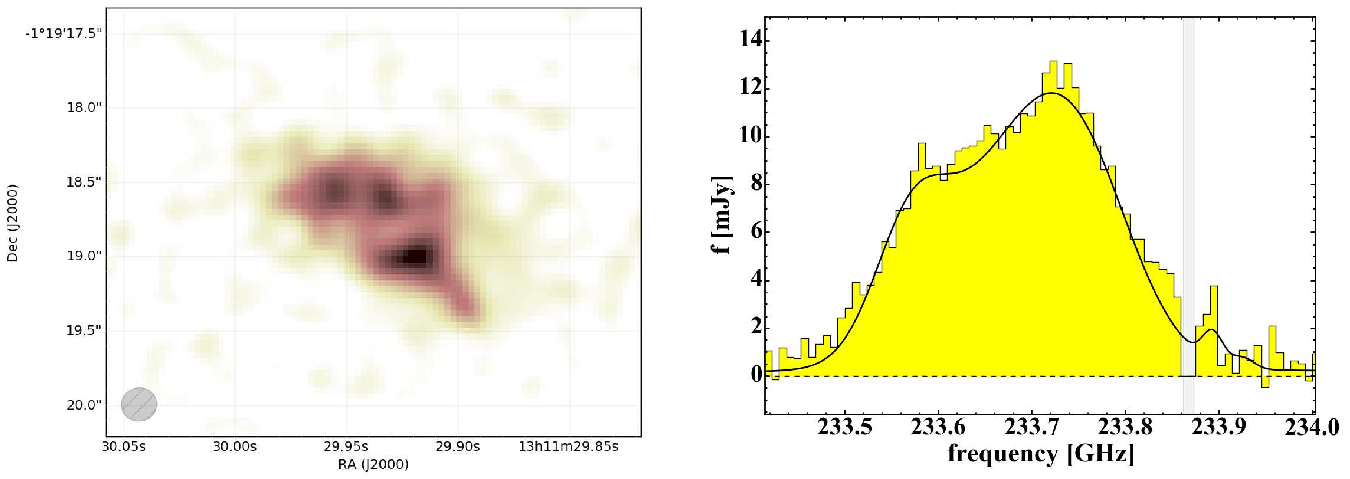
\includegraphics[width=1.0\textwidth,clip=]{ALMA_14.pdf}
  \caption{ALMA Cycle~3 data in band 6 showing an image (\emph{left}) and the
           spectrum (\emph{right}) in the emission line
           [C\,\textsc{ii}]\,157.7\,$\mu$m. The redshift is \(z=7.132\).
           (The light grey box indicates flagged channels.)}
\end{figure}

\clearpage

\bibliography{z7_alma}

\clearpage

\section{Technical Remarks (2 pages max)}

\subsection{The need for Keck/MOSFIRE}

There are very few instruments in the world capable of detecting the wing at
this redshift.  We require an 8--10\,m-class telescope because the target is so
faint, and we require an efficient detector at 1000\,nm. We have deep X-shooter
data for this target, but in this specific band \(990-1030\)\,nm, where the
X-shooter dichroic lies, X-shooter has a factor of 2--3 dip in efficiency due to
the low sensitivity of first and last spectral orders of the NIR and VIS arms
respectively. However, MOSFIRE'S \(Y\) grating has the sensitivity to make this
observation.


\subsection{Targets and Exposures:}

The target is A1689-zD1, R.A. 13 11 29.93, Dec. \(-\)01 19 18.7. It has a
\(M_{J_{\rm AB}} = 25\) Source extent is \(1^{\prime\prime}\). The requested
exposure time is 16 hours.

The required time is calculated based on detecting the shape of a \lya\ damping
wing with a width of \(\sim40\)\,nm.  We require 10 bins across the wing, i.e.\
4\,nm per bin, with a SNR \(\sim3\).  The MOSFIRE ETC for a \(Y_{\rm
AB}=25.0\)\,mag source (the HST F125W detection was \(25.0\pm0.13\) and the
spectrum is flat in F\(_\nu\)), extended over 1\,square arcsecond area (Watson
et~al. 2015) with a slit width of \(0.7^{\prime\prime}\) gives a time required of about
50000\,s. A SNR=0.6/pixel is found for the integrated source and 0.109\,nm/pixel
spectral dispersion in a 16 hour total exposure time with 1200\,s integrations.
This corresponds to a SNR over a 4\,nm bin of \(\sim3.6\) taking into account
that approximately half of the spectral band is heavily affected by sky emission
lines. We used the MOSFIRE ETC with model galaxies, one cutoff at
\(z=7.132\) (Meiksin 2006) and one with a \(\log(N_{{\rm H\,I}}/{\rm
cm}^2)=23.1\) DLA, to represent the IGM, at \(z=7.132\), and determined the SNR
spectrum, which includes instrument and sky emission and absorption
contributions.

From these SNR spectra we simulated the output spectra and we show these
simulations in Fig.~1 (right). Based on these simulations we can clearly
discriminate between a break and a damping wing at \(z=7.13\) with 16 hours on
source exposure. We can also fit the damping wing to measure the column density.

To remove the background and optimize the SNR on our high-redshift object we
will adopt the following strategy. We will nod along the slits, using a
telescope nodding sequence ABAB with 1200\,s exposure each. This will optimize
the sky subtraction and maximize the science exposure, since the science target
is observed 100\% of the time.

The remaining slits will be used to observe photometrically selected lensed
galaxies at typically \(z=1 - 1.5\). At those redshifts we will target [\oiii],
[\oii] and H\textbeta. Given the significant exposure time for many of them we
will be able not only to determine redshift but also to derive meaningful
spatially resolved information and dynamical properties.

Lunar phase: This is a very faint target, but NIR observations only are
required, so grey time is acceptable.

\subsection{Backup Program:}

If conditions are too poor to target very faint galaxies at \(z > 7\), we will
instead observe brighter, relatively low-redshift galaxies in the CANDELS UDS,
GOODS-S and COSMOS fields, which are available in a similar range of right
ascensions.   We we will observe  H\textalpha\ + [NII] (and if possible also
[SII] for galaxies at \(0.4 < z < 1\), where we already  have [OIII]+H\textbeta\
measurements from existing optical spectra, in order to measure line  excitation
diagnostics (BPT diagrams).   These will be used to calibrate alternate methods,
such as the Mass-Excitation (MEx) diagram of Juneau et al.\ 2011, that can be
applied at high redshift without the need for infrared spectroscopy.  Other
programs, such as measuring nebular line extinction from the Balmer decrement
for infrared-luminous galaxies with detections in deep Herschel and Spitzer
data, will also be pursued to the extent that we can assess the relative
H\textalpha\ to H\textbeta\ flux calibration, using continuum detections of the
galaxies to compare with HST photometry (and morphology to assess slit losses).

\subsection{Supplementary Observations:}
No other observations are required.

\subsection{Status of Previously Approved Keck Programs (B. Mobasher):}
\begin{itemize}
  \item ``The MOSDEF Survey'' (co-PIs Shapley/Kriek/Reddy/Siana/Coil/Mobasher):
        This LMAP program was allocated 45.5 nights. Data from all the runs have
        been reduced and analyzed and used. Early data are included in MOSDEF
        publications. Because of this, B.~Mobasher did not submit proposals in
        2013A-2015A.
  \item Search for \(z\sim7.7\) and 8.8 galaxies in the DAWN fields---Mobasher 1.5
        nights 2015B MOSFIRE:\ lost 1 night to weather, need more exposure on the
        sources to publish.
  \item	Nature and Dynamics of Kpc-scale Clumps in star forming disk galaxies at
        \(1 < z < 2\)---Mobasher OSIRIS 1.5 nights: Lost one night to weather.
        Found no signature of H\textalpha/H\textbeta\ lines we were looking for
        in the two target galaxies.
  \item	Evidence for Population III Light from a Galaxy at z=6.6: 2 nights of
        DEIMOS:\ time 2015B. Clear weather. Results published in Sobral et~al.
        2016.
  \item	Spectroscopic Observations of Galaxies in the Cosmic web: 1.5 nights
        DEIMOS:\ December 2016 weathered out.
\end{itemize}

\clearpage

\section{Optional, but highly recommended, subsections (2 pages max)}

\subsection{Path to Science from Observations:}

The observations will be carried out by Mobasher or Nayyeri. The data will be
reduced and analyzed by our team, led by Mobasher, Watson, and Nayyeri. The
analysis and reduction of the other targets in the field, which are primarily
multiply-imaged systems, will be done by Johan Richard and Kirsten Knudsen. An
improved mass model for Abell\,1689 will be derived from these data, and
constraints determined on background SMGs.

\subsection{Technical Concerns:}

The observations proposed here, while very deep, are not complex, and should be
achievable with a straightforward observing strategy. The most important thing
is to get a good sky subtraction. The simple ABBA nodding scheme proposed here
should be good enough to achieve an accurate subtraction.

\subsection{Publications by the Principal Investigator:}

Some publications relevant to the present proposal (work based on Keck data is marked with *):
\begin{enumerate}
  \item Nayyeri H., Mobasher B., et al. 2014 ``A Study of Massive and Evolved Galaxies at
        High Redshift'', ApJ 794, 68;
  \item * Mobasher B., et al. 2015, ``A Critical Assessment of Stellar Mass Measurement
          Methods'', ApJ 808, 101;
  \item * Sobral D., Matthee J., Darvish B., Schaerer D., Mobasher B., et al. 2015 ``Evidence
          for PopIII-like Stellar Populations in the Most Luminous Lyman-Emitters at the
          Epoch of Reionization: Spectroscopic Confirmation'', ApJ 808, 139;
  \item * Khostovan A. A., Sobral D., Mobasher B., et al. 2016 ``The nature of H\textbeta+[OIII]
          and [OII] emitters to z = 5 with HiZELS: stellar mass functions and the evolution of
          EWs'', MNRAS 463, 2363;
  \item * Faisst, A. L., [\ldots], Mobasher B. et al. 2016 ``Rest-UV Absorption Lines as Metallicity
          Estimator: The Metal Content of Star-forming Galaxies at z~5'', ApJ 822, 29;
  \item * Darvish B., Mobasher B., et al. 2016 ``The Effects of the Local Environment and
          Stellar Mass on Galaxy Quenching to \(z \sim 3\)'', ApJ 825, 113; 7
  \item * Nayyeri H., Hemmati S., Mobasher B., Ferguson H. C. et al. 2017 ``CANDELS
          Multi-wavelength Catalogs: Source Identification and Photometry in the CANDELS
          COSMOS Survey Field'', ApJS 228, 7;
  \item * Khostovan A. A., Sobral D., Mobasher B., et al. 2018 ``The clustering of H\textbeta+[OIII]
          and [OII] emitters since \(z \sim 5\): dependencies with line luminosity and stellar mass'',
          MNRAS 478, 2999.
\end{enumerate}

Co-Is Watson and Knudsen have been leading ESO observations of this galaxy and
published the first spectroscopic redshift and ALMA detections.

\noindent \smallskip\\
Watson D. et~al., 2015, Nature, 519, 327: A dusty, normal galaxy in the epoch of reionization
\smallskip\\
Knudsen K.~K. et~al., 2017, MNRAS 466, 138: A merger in the dusty, z = 7.5 galaxy A1689-zD1?

\subsection{Resources and Publication Timescale:}

The primary result---the detection of the Gunn-Peterson damping wing, will be
written up rapidly in the first instance for publication in a high impact
journal without extensive modelling. Watson and Nayyeri will be available to do
this, with a first draft quickly, about two months after the observations since
the observations will likely be performed in March--May, after the main teaching
season. A follow-up paper will be written, modelling the IGM neutral fraction
constraints with assistance from J.~Zavala. The timescale for this is longer,
about 6 months after the first publication. The publication of the revised mass
constraints on Abell\,1689 and the sub-mm galaxies depends on the level of
improvement that can be derived from the data, but are likely to be part of a
larger publication within 18 months of the observations.

\subsection{Service to UCO (new since 2017B):}
The PI is the IRMS instrument scientist on the TMT. He has developed
preliminary exposure time calculator for the IRMS and performed a
study of the capabilities of this instrument. The PI is also PI of a
\$4.5M grant from NASA to perform research and training in Big Data.
This will provide the funding for a graduate student to work on the
project proposed here. The PI has been supporting a significant number
of undergraduate students from different UC campuses as well as a
number of graduate students at UCR through his NASA-MIRO grant.

\end{document}
